% AutoPlay -- IEEE conference paper (IEEEtran v1.8b, conference mode).
% DRAFT: Section IX contains placeholders that MUST be replaced by device
% measurements before submission. Do not submit with \tbm cells remaining.
\documentclass[conference]{IEEEtran}
\IEEEoverridecommandlockouts

\usepackage{cite}
\usepackage{amsmath,amssymb}
\usepackage{graphicx}
\usepackage{booktabs}
\usepackage{tabularx}
\usepackage{array}
\usepackage{xcolor}
\usepackage{tikz}
\usetikzlibrary{arrows.meta,positioning,decorations.pathreplacing}
\usepackage[hyphens]{url}
\usepackage[hidelinks]{hyperref}

\newcommand{\tbm}{\textcolor{red}{\textit{TBM}}}
\newcommand{\draftnote}[1]{\textcolor{red}{#1}}
\newcolumntype{L}[1]{>{\raggedright\arraybackslash}p{#1}}
\newcolumntype{Y}{>{\raggedright\arraybackslash}X}

\begin{document}

\title{Clock-Free, Authenticated Playback Handoff\\Between Android Phones Sharing Multipoint Earbuds}

\author{\IEEEauthorblockN{Keshav Gehlot}
\IEEEauthorblockA{\textit{Department of Networking and Communications}\\
\textit{SRM Institute of Science and Technology}\\
Kattankulathur, Chennai, India\\
kg0998@srmist.edu.in}}

\maketitle

\begin{abstract}
A listener who carries two Android phones and one pair of multipoint Bluetooth earbuds must still stop the music on one phone and find it again on the other. Platform continuity features, such as Apple's Handoff and Android~17's Continue On, offer to resume an app's own activity on another of the user's devices when the user picks it up there; they do not arbitrate which device plays, and published analyses of one such protocol and of Android's Nearby Connections transport report denial-of-service, tracking and relay attacks. We present AutoPlay, an application-layer protocol that hands a playback session from one phone to another while keeping at most one phone playing. The target plays under a provisional lease anchored on its own READY message and only the source commits or aborts, so safety rests on bounded timer drift rather than synchronised clocks. A nonce echo and a memory of finished transactions reject delayed duplicates. A companion security layer closes gaps identified in two published protocol analyses with pinned device identities, a handshake bound to the transport's connection token, and a replay window that only authenticated messages can move. We implement the protocol in Kotlin and evaluate it by fault injection over nearly 18 million simulated handoff attempts. Under message loss up to 30\%, link outages, clock skew up to 10\,s and coordinator crashes, the safe-pause variant produced no dual playback in 3.45 million faulty attempts, against 0.65\% for an expiry-based design and 0.86\% for a naive one. Wall-clock expiry completed 55.8\% of handoffs at 5\,s skew, where the lease completed 94.9\%. No forged, replayed or relayed message was accepted in 2.3 million attempts. \draftnote{Device measurements are in progress and are not reported in this draft.}
\end{abstract}

\begin{IEEEkeywords}
Bluetooth, multipoint audio, session handoff, leases, Nearby Connections, protocol security, fault injection, Android
\end{IEEEkeywords}

% =====================================================================
\section{Introduction}

Multipoint earbuds keep links to two phones, yet moving a song from one phone to the other remains manual: pause, pick up the second phone, open the player, find the track and the position. The headset arbitrates the audio link; nothing arbitrates the playback session.

Vendors address parts of this inside their own ecosystems. Apple's Handoff resumes an activity on a second device logged in to the same iCloud account~\cite{stute2021}. Android~17 (API level~37) added a Handoff API, presented to users as Continue On: an app specifies state to be resumed, and the system shows a handoff suggestion in the launcher of the user's nearby devices~\cite{android17,continueon}; at launch it supports phone-to-tablet transitions~\cite{continueon}. In both, an app opts in to hand off its own state and the user acts on a suggestion at the receiving device; neither decides which of two phones should be playing.

A third-party coordinator faces three problems that these features do not. First, it must keep at most one phone playing although it controls neither the music app nor the headset, and although messages between the phones are lost, delayed and duplicated. Second, it cannot assume the phones' clocks agree. Third, in the version analysed by Antonioli et al., its practical local transport on Android, Nearby Connections, left peer authentication optional, relied on a short token compared by users, and did not enforce proximity~\cite{antonioli2019}.

This paper makes four contributions:
\begin{enumerate}
\item A two-party handoff protocol in which the target plays under a provisional lease anchored on its own READY message and the source alone commits or aborts. Safety requires bounded timer drift, not clock synchronisation (Section~\ref{sec:protocol}).
\item A gap analysis of two published protocol studies~\cite{stute2021,antonioli2019} and a security layer that closes the gaps an application can close (Sections~\ref{sec:base} and~\ref{sec:security}).
\item A Kotlin implementation with a fault-injection simulator, to be released with the paper, and an ablation over nearly 18 million handoff attempts that isolates what each mechanism prevents (Section~\ref{sec:faulteval}).
\item The identification of a hazard specific to coordinating a player one does not own: when the coordinator process dies, the player keeps playing. We show that automatic rollback is unsafe under this fault and quantify the cost of the safe alternative.
\end{enumerate}

\draftnote{This draft reports no results from physical devices; Section~\ref{sec:hw} lists the measurements that remain.}

% =====================================================================
\section{System and Threat Model}\label{sec:model}

\textbf{System.} Two phones, A and B, each run a coordinator and a music player that the coordinator can ask to pause, seek and play. Both phones are bonded to one multipoint headset. The coordinator can observe whether the headset is a current audio output but cannot command the headset. The phones exchange messages over a local link.

\textbf{Faults.} Messages may be lost, delayed without bound, duplicated and reordered; the link may fail for seconds. Wall clocks may differ by any amount, and local timers drift at a bounded rate. The coordinator process may stop and later restart with its persisted state; while it is stopped, the player keeps its state. Player commands complete after a bounded delay, and a start may fail.

\textbf{Safety property.} At no instant are both players audibly playing the managed session for longer than a tolerance, set to 100\,ms in our evaluation.

\textbf{Liveness goal.} After a handoff attempt, exactly one phone plays without user action as often as the faults allow.

\textbf{Adversary.} An attacker within radio range, or relaying to it, who can run the transport protocol, open connections to either phone, and inject, drop, delay, replay and modify messages, but holds no enrolled identity key. The attacker aims to play or pause the victim's audio, cause dual playback, block handoffs persistently, learn what is playing, or track the user through the application's identifiers.

\textbf{Out of scope.} A compromised or stolen enrolled phone; attacks on Bluetooth pairing and link keys themselves~\cite{bias2020,bluffs2023,blurtooth2020,happymitm2021,stealtooth2025}; jamming; and the music service's account security.

% =====================================================================
\section{Literature Survey}\label{sec:related}

We found no peer-reviewed work on automatic playback handoff between phones that share a headset. Table~\ref{tab:survey} summarises the nearest work in six themes.

\textbf{Search method and limits.} Searches were run in November 2026 with a general web search engine and a research-paper index covering arXiv and biomedical literature, covering Bluetooth multipoint and audio handover, continuity-protocol security, Nearby Connections, session and task migration, leases and fencing, media synchronisation, and Bluetooth proximity. IEEE Xplore, the ACM Digital Library and Scopus were not searched directly and no patent search was done, so the absence claim is provisional. \draftnote{[Complete these searches before submission.]}

\begin{table*}[t]
\caption{Surveyed Work and Its Limits for Exclusive Playback Handoff}
\label{tab:survey}
\centering
\footnotesize
\begin{tabularx}{\textwidth}{@{}L{2.2cm}L{3.4cm}YY@{}}
\toprule
\textbf{Theme} & \textbf{Work} & \textbf{Finding} & \textbf{Limit for this problem} \\
\midrule
Continuity protocols & Stute et al.~\cite{stute2021} & Tracking, DoS and MitM attacks on Apple Handoff, Universal Clipboard and Wi-Fi Password Sharing & Vendor protocol tied to one cloud account; user-initiated; no playback arbitration \\
 & Martin et al.~\cite{martin2019} & Continuity BLE messages leak device and behavioural data; predictable sequence numbers defeat address randomisation & Privacy analysis only \\
 & Heinze et al.~\cite{heinze2020} & MagicPairing lets a peripheral paired once be used with all of a user's Apple devices; fuzzing found implementation flaws & Requires vendor control of the peripheral and ecosystem \\
\midrule
Local transport & Antonioli et al.~\cite{antonioli2019} & Security analysis of Nearby Connections (Play Services 12.8.74); connection-manipulation and range-extension attacks & Proposes no countermeasures \\
 & Yair and Cohen~\cite{quickshell2024} & Ten vulnerabilities in Google's Quick Share, including a forced Wi-Fi connection & Not peer reviewed; file-transfer app \\
\midrule
Bluetooth link security & \cite{bias2020,bluffs2023,blurtooth2020,happymitm2021,stealtooth2025} & Impersonation, broken session secrecy, cross-transport key abuse, missing key-change warnings, silent key overwrite & The link under an application cannot be assumed authenticated \\
 & Gasteiger et al.~\cite{bison2023} & Attack on broadcast isochronous streams exploiting plaintext synchronisation metadata & Broadcast audio, not multipoint \\
\midrule
Session migration & Shacham et al.~\cite{shacham2007,rfc5631} & SIP-based transfer of multimedia sessions between nearby devices & Needs SIP endpoints and control of the stream \\
 & Flux~\cite{flux2015} & Migrates unmodified Android apps between devices using record and replay & Requires its Android-based system on both devices \\
 & Deep Shot~\cite{deepshot2011} & Moves application state between devices via a camera-captured URI & User-initiated; apps must expose state \\
 & Brudy et al.~\cite{brudy2019} & Taxonomy of 510 cross-device interaction papers & Survey; no protocol \\
\midrule
Exclusive ownership & Gray and Cheriton~\cite{gray1989} & Leases: time-limited rights that handle host and communication failures using physical clocks & Client--server caching; basis of our lease \\
 & Chubby~\cite{chubby2006} & Lock service; sequencers carrying a lock generation number let servers reject stale holders & Needs a replicated service \\
 & Raft~\cite{raft2014} & Consensus with majority quorums & Two phones have no majority under partition \\
\midrule
Media sync. & \cite{montagud2012,rfc7272} & Synchronised playout at several receivers & Handoff needs mutual exclusion, not synchrony \\
\midrule
Proximity & Faragher and Harle~\cite{faragher2015} & BLE fingerprinting; RSSI is highly susceptible to fast fading & Needs beacon infrastructure \\
 & Leith and Farrell~\cite{leith2020} & On a bus, reported attenuation need not increase with distance; detection rate depended only weakly on distance & Signal strength alone cannot trigger handoff \\
\bottomrule
\end{tabularx}
\end{table*}

Three observations follow. Work on continuity protocols and on Nearby Connections analyses existing protocols rather than designing safer ones. Migration systems assume they own the application or the stream, which a coordinator of a commercial music app does not. Ownership mechanisms assume servers or quorums that two phones lack, which leaves leases as the applicable tool.

% =====================================================================
\section{Base Papers and Gap Analysis}\label{sec:base}

We take as base papers the most complete public analysis of a deployed handoff protocol~\cite{stute2021} and the only peer-reviewed analysis we found of the transport AutoPlay uses~\cite{antonioli2019}.

\textbf{Base paper A~\cite{stute2021}.} Stute et al.\ reverse-engineer three Apple Continuity services. Handoff uses BLE advertisements encrypted with AES-GCM under a dedicated key with a linearly increasing counter as IV, discovery over mDNS on AWDL, and an authenticated exchange whose long-term public keys are synchronised through the iCloud keychain; the devices must be logged in to the same iCloud account. The advertisement IV is 2\,bytes and the tag 1\,byte, and a receiver accepts only an IV higher than the last accepted one. By spoofing the sender's address and sending 256 advertisements with the maximum IV, one per tag value, an attacker advances the receiver's stored IV; later legitimate advertisements are dropped until reboot. The linearly increasing IV and identifiers that are not randomised synchronously also enable tracking. The authors recommend adding a longer (64-bit) tag, a shuffled IV sequence, and synchronised identifier rotation.

\textbf{Base paper B~\cite{antonioli2019}.} Antonioli et al.\ reverse-engineer Nearby Connections in Google Play Services~12.8.74. Peer authentication is optional and consists of a five-character token that users are expected to compare; the paper notes that Google's sample code ignores it. The Bluetooth link key is neither authenticated nor persistent, and each connection's key exchange yields fresh secrets. The authors impersonate endpoints, interpose between victims, force a victim onto an attacker-controlled access point, and tunnel a connection between devices that are not near each other. The paper proposes no explicit countermeasures.

\textbf{Gaps.} Table~\ref{tab:gaps} lists the gaps and our response. G4 is a gap relative to our problem rather than a flaw in Handoff, which is designed for user-chosen continuation and reports no exclusivity guarantee.

\begin{table}[t]
\caption{Gaps in the Base Papers and AutoPlay's Response}
\label{tab:gaps}
\centering
\footnotesize
\begin{tabularx}{\columnwidth}{@{}L{0.45cm}YYL{0.6cm}@{}}
\toprule
 & \textbf{Gap (source)} & \textbf{Response} & \textbf{Sec.} \\
\midrule
G1 & Short-tag forgery advances replay state; handoffs blocked until restart (A) & 128-bit tag; window moves only after authentication & \ref{sec:security}, \ref{sec:seceval} \\
G2 & Counters and unaligned identifiers enable tracking (A) & No plaintext counter; identifiers from one epoch & \ref{sec:security} \\
G3 & Trust rooted in a vendor cloud account (A) & Local enrolment, pinned keys, no server & \ref{sec:security} \\
G4 & No arbitration of which device continues (A) & Epoch-fenced owner, provisional lease & \ref{sec:protocol}, \ref{sec:faulteval} \\
G5 & Authentication optional, per-connection, user-mediated (B) & Mutual signatures, pinned identities & \ref{sec:security}, \ref{sec:seceval} \\
G6 & Authentication only by a per-connection token (B) & Long-term device keys and roster & \ref{sec:security} \\
G7 & MitM and range extension across two connections (B) & Transport token bound into signed handshake & \ref{sec:security}, \ref{sec:seceval} \\
G8 & Proximity not enforced (B) & Target attests its own headset route; short windows & \ref{sec:protocol} \\
G9 & Fixes addressed to the vendor (A) or none (B); none for third-party apps & Implementation and adversarial tests & \ref{sec:impl}--\ref{sec:seceval} \\
\bottomrule
\end{tabularx}
\end{table}

% =====================================================================
\section{Handoff Protocol}\label{sec:protocol}

The protocol is break-before-make with a provisional lease: the source pauses, the target plays for at most a window $W$ unless committed, and only the source decides the outcome. Each phone stores the highest committed owner epoch and its owner. A handoff is a transaction with a random identifier \textit{tx} and the epoch it would create. Fig.~\ref{fig:seq} shows a successful run and Table~\ref{tab:msgs} the message set.

\begin{figure}[t]
\centering
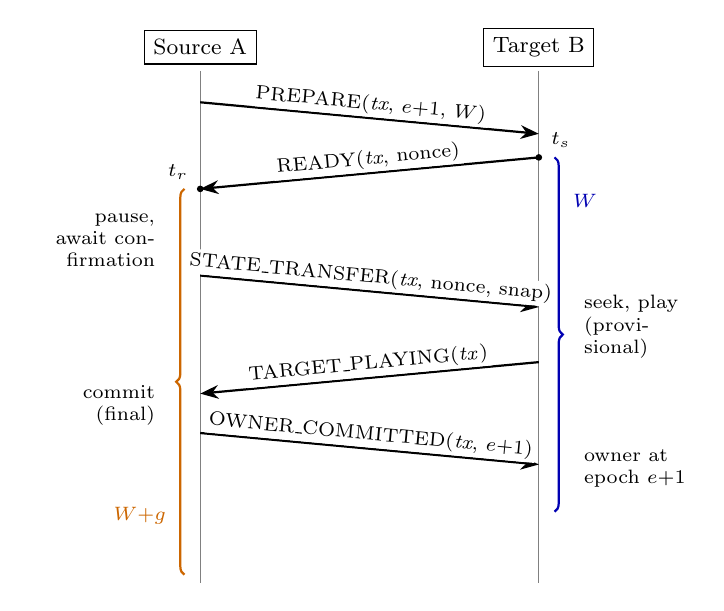
\begin{tikzpicture}[>=Stealth, font=\scriptsize,
  msg/.style={->, thick},
  lab/.style={fill=white, inner sep=1pt}]
  \def\xa{0} \def\xb{4.3}
  \node[draw, minimum width=1.4cm, font=\footnotesize] at (\xa,0) {Source A};
  \node[draw, minimum width=1.4cm, font=\footnotesize] at (\xb,0) {Target B};
  \draw[gray] (\xa,-0.3) -- (\xa,-6.8);
  \draw[gray] (\xb,-0.3) -- (\xb,-6.8);
  \draw[msg] (\xa,-0.7) -- node[lab, above, sloped] {PREPARE(\textit{tx}, $e{+}1$, $W$)} (\xb,-1.1);
  \draw[msg] (\xb,-1.4) -- node[lab, above, sloped] {READY(\textit{tx}, nonce)} (\xa,-1.8);
  \fill (\xb,-1.4) circle (1.2pt) node[above right=0pt and 1pt] {$t_s$};
  \fill (\xa,-1.8) circle (1.2pt) node[above left=0pt and 1pt] {$t_r$};
  \node[left, align=right, text width=1.5cm] at (\xa-0.45,-2.45) {pause, await confirmation};
  \draw[msg] (\xa,-2.9) -- node[lab, above, sloped] {STATE\_TRANSFER(\textit{tx}, nonce, snap)} (\xb,-3.3);
  \node[right, align=left, text width=1.3cm] at (\xb+0.45,-3.55) {seek, play (provisional)};
  \draw[msg] (\xb,-4.0) -- node[lab, above, sloped] {TARGET\_PLAYING(\textit{tx})} (\xa,-4.4);
  \node[left, align=right, text width=1.5cm] at (\xa-0.45,-4.55) {commit (final)};
  \draw[msg] (\xa,-4.9) -- node[lab, above, sloped] {OWNER\_COMMITTED(\textit{tx}, $e{+}1$)} (\xb,-5.3);
  \node[right, align=left, text width=1.3cm] at (\xb+0.45,-5.35) {owner at epoch $e{+}1$};
  % window W on B: from t_s; lease W+g on A: from t_r, ends later
  \draw[decorate, decoration={brace, amplitude=3pt}, thick, blue!70!black] (\xb+0.2,-1.4) -- (\xb+0.2,-5.9)
    node[midway, right=3pt, rotate=0, yshift=17mm] {$W$};
  \draw[decorate, decoration={brace, amplitude=3pt, mirror}, thick, orange!80!black] (\xa-0.2,-1.8) -- (\xa-0.2,-6.7)
    node[midway, left=3pt, yshift=-17mm] {$W{+}g$};
\end{tikzpicture}
\caption{A successful handoff. B's window starts when B \emph{sends} READY ($t_s$); A's lease starts when A \emph{receives} it ($t_r \ge t_s$). B stops itself at the end of $W$ unless committed; A may abort only after $W+g$.}
\label{fig:seq}
\end{figure}

\begin{table}[t]
\caption{Protocol Messages}
\label{tab:msgs}
\centering
\footnotesize
\setlength{\tabcolsep}{4pt}
\begin{tabularx}{\columnwidth}{@{}>{\scriptsize\raggedright\arraybackslash}p{2.55cm}L{0.72cm}Y@{}}
\toprule
\textbf{Message} & \textbf{Dir.} & \textbf{Meaning} \\
\midrule
PREPARE & A$\to$B & Request handoff at a new epoch with window $W$ \\
READY & B$\to$A & B is idle, routed to the headset, window started; carries a nonce \\
REJECTED & B$\to$A & Stale epoch, not owner, busy, no route, or user override \\
STATE\_TRANSFER & A$\to$B & A is paused; play this content at this position; echoes nonce \\
TARGET\_PLAYING & B$\to$A & B plays provisionally \\
OWNER\_COMMITTED & A$\to$B & A committed; B owns the session \\
ABORT\_REQ & A$\to$B & Stop and confirm \\
ABORTED & B$\to$A & B is not playing \textit{tx} and never will \\
RECOVERY\_QUERY & B$\to$A & B stopped at window end; asks the decision \\
OWNER\_CLAIM & either & User pressed play here; new epoch \\
\bottomrule
\end{tabularx}
\end{table}

\subsection{Timing Rules}

Let $t_s$ be the instant B sends READY, on B's timer, and $t_r$ the instant A receives it, on A's timer. Let $b_{\mathrm{start}}$ and $b_{\mathrm{pause}}$ bound the player's start and pause latencies and $g$ be a guard.

\begin{itemize}
\item[R1] B starts playback only on a STATE\_TRANSFER that echoes its nonce and arrives before $t_s + W - b_{\mathrm{start}}$.
\item[R2] Unless it has received OWNER\_COMMITTED, B issues a pause at $t_s + W - b_{\mathrm{pause}}$ and then sends RECOVERY\_QUERY.
\item[R3] A takes the snapshot only after its own pause is confirmed.
\item[R4] A commits on the first TARGET\_PLAYING, or a RECOVERY\_QUERY reporting that B had started, received before $t_r + W + g$; after that it decides abort. Either decision is final.
\item[R5] Under the \emph{rollback} policy A resumes when it decides abort. Under \emph{safe-pause} it resumes only on receiving ABORTED.
\item[R6] Each phone remembers finished transactions and rejects messages that refer to them.
\end{itemize}

Our implementation uses $W=4$\,s, $g=0.5$\,s, $b_{\mathrm{start}}=1$\,s, $b_{\mathrm{pause}}=0.3$\,s and a 250\,ms retransmission interval. \draftnote{These values are provisional and will be set from measured P99 player latencies.}

\subsection{Safety Argument}

Assume that B's coordinator runs, that a pause completes within $b_{\mathrm{pause}}$, and that timers drift by less than $g$ over $W$. By R1 and R2, B is silent after $t_s+W$ unless committed. A message cannot be received before it is sent, so $t_r \ge t_s$ in real time, and by R4 A decides abort no earlier than $t_s + W + g$ less drift, which is after B is silent. If A commits instead, R4 makes the decision final and A never resumes. Hence the players do not overlap. The argument compares two durations that start at causally ordered events and never compares the phones' clocks. It adapts the lease of Gray and Cheriton~\cite{gray1989} to a two-party ownership transfer, with the holder's term starting when it sends READY and the grantor's when it receives it.

\textbf{The orphaned-player hazard.} If B's coordinator process dies inside the window, R2 does not execute and the music app keeps playing. Under rollback, A then resumes while B plays. Under safe-pause, A stays silent until B restarts, pauses its player and answers. Section~\ref{sec:faulteval} measures both policies.

\textbf{Freshness.} Without the nonce of R1, a delayed PREPARE and STATE\_TRANSFER of an aborted transaction can arrive in order after A has resumed, and B would start. The nonce ties a transfer to the READY of the current attempt; R6 covers transactions B has already seen.

\textbf{User intent.} A manual pause cancels a pending transaction and suspends automation. A manual play claims a new epoch; the other phone pauses on receiving the claim.

% =====================================================================
\section{Security Layer}\label{sec:security}

The security layer treats Nearby Connections as an untrusted pipe and places identity, key agreement and replay protection above it.

\textbf{Enrolment (G3, G6).} Each phone holds an ECDSA P-256 identity key; on Android it is to be generated in the platform keystore, while our JVM prototype keeps it in memory. Two phones enrol once, held by the same user: each scans a QR code of the other's key fingerprint, or the user compares a six-digit short authentication string computed after a commit-then-reveal exchange of nonces. The result is a pinned roster; no server or account is involved.

\textbf{Session handshake (G5, G7).} For each transport connection the phones run a three-message signed Diffie--Hellman exchange: ephemeral P-256 keys and nonces are exchanged, and each side signs a hash of the transcript with its identity key. Because the transcript names both identities, the identity bound to the session is the one that signed, the property SIGMA~\cite{sigma2003} was designed to ensure; our exchange has not been formally verified. The transcript also includes the hash of the transport's raw authentication token for that connection, which Nearby Connections exposes for programmatic authentication~\cite{nearbydocs}. An attacker who terminates a separate connection with each victim holds two different tokens, so neither victim's signature verifies at the other, and no user comparison is needed. Per-direction keys and a session identifier are derived with HKDF-SHA-256~\cite{rfc5869} from the ECDH secret, both nonces and the transcript hash.

\textbf{Message protection (G1).} Each message is sealed with AES-256-GCM under the direction key with a 128-bit tag, in line with base paper~A's own recommendation of a longer tag. The nonce is a 64-bit sequence number, and the associated data binds the session identifier, sender, recipient and sequence number. The receiver keeps a 64-entry sliding window. It checks the window without changing it, verifies the tag, and only then marks the sequence number as seen. A forgery cannot move the window, whatever sequence number it carries, so the desynchronisation of base paper~A has no counterpart. Separate direction keys make reflected frames fail.

\textbf{Identifiers (G2).} The endpoint name, the one advertised identifier the application chooses, is a truncated HMAC of a group key and a 15-minute epoch index. Members recompute it; without the key, two epochs' names cannot be linked. Sequence numbers exist only inside the encrypted link. Identifiers emitted by Nearby Connections itself, such as its service and endpoint identifiers, are outside the application's control.

\textbf{Proximity (G8).} Reachability is never treated as nearness. B answers READY only if its own audio device list shows the enrolled headset connected as an output, which places B within Bluetooth range of the headset, and all deadlines are short relative windows that bound the age of a relayed message.

\textbf{Residual risk.} A relay that forwards a single connection at the radio layer preserves the token and passes the handshake; distance bounding would be needed to stop it. Such an attacker can delay and drop messages but cannot read, forge or replay them, and by Section~\ref{sec:protocol} delay and loss do not cause dual playback.

% =====================================================================
\section{Implementation}\label{sec:impl}

The protocol and security layer form a dependency-free Kotlin module of 925 lines; with the simulator and tests the code totals 1{,}895 lines and builds with kotlinc~2.1.21 on JDK~21. The coordinator is a deterministic state machine of ten phases that reaches the outside world through three interfaces: an environment (monotonic time, timers, send), a player port (asynchronous pause and play with completion callbacks, and a snapshot) and a route predicate. On Android these map to \texttt{SystemClock.elapsedRealtime}, a playback adapter and the audio device list; in tests they are simulated, so the coordinator evaluated in the simulator is the code intended to run on the phone. A state-transfer message is 110\,bytes encoded and 135\,bytes sealed. The design writes state to stable storage before each transition takes effect, so a restarted coordinator can stop an uncommitted provisional playback; the simulator models this by preserving coordinator state across crashes. Enrolment helpers are implemented; the enrolment user interface is not.

The Android application, the Nearby Connections binding, the route observer and the playback adapters are \draftnote{not yet implemented}. Three adapters are planned: a Media3 reference player that plays an identical test asset on both phones and provides position ground truth; a Spotify App Remote adapter, whose testing is limited by Spotify's February 2026 Development Mode changes, which require the developer to hold Premium and cap each app at five users~\cite{spotify2026}, and by the SDK's requirement of a Premium account to play a single track~\cite{spotifysdk}; and an experimental adapter over Android media sessions.

% =====================================================================
\section{Evaluation by Fault Injection}\label{sec:faulteval}

\textbf{Method.} A discrete-event simulator drives two coordinators, two players and a lossy link. Each trial makes three handoff attempts spaced 22\,s apart plus a random offset of up to 2\,s. A checkpoint 16\,s after each trigger records which phones play; if not exactly one, a simulated user presses play on the target. For a given seed every variant sees the same outage, crash and clock schedule; per-message loss and delay are drawn as messages are sent and therefore differ between variants. Each setting runs 50{,}000 trials (150{,}000 attempts), over 23 fault settings and a fault-free setting.

\textbf{Fault model.} Loss is independent per message. Delay is log-normal with a 30\,ms median, and 3\% of messages take an extra 0.5--6\,s; 3\% are duplicated and 1\% are duplicated again after 5--40\,s. An outage lasts 1.5--12\,s and starts within 1.5\,s of the trigger. A coordinator crash starts within 3\,s of the trigger and lasts 2--8\,s, with the player keeping its state. Wall clocks are offset uniformly within the skew bound and timers drift by up to 100\,ppm. Player commands take 30--300\,ms and 5\% of target starts fail. Unless swept, loss is 5\%, skew $\pm$1\,s, outage probability 10\% and crash probability 2\% per phone.

\textbf{Variants.} A0 pauses, transfers and rolls back on an acknowledgement timeout. A1 adds PREPARE/READY, owner epochs, finished-transaction memory and a wall-clock expiry; its target commits on start, and conflicts are reconciled by epoch. A2 is the protocol of Section~\ref{sec:protocol} with rollback, A3 with safe-pause, and A2$^-$ is A2 without the nonce and transaction memory.

\begin{table}[t]
\caption{Default Fault Setting (150{,}000 Attempts per Variant)}
\label{tab:default}
\centering
\footnotesize
\begin{tabular}{@{}lccccc@{}}
\toprule
\textbf{Variant} & \textbf{Handed} & \textbf{Kept} & \textbf{Dual} & \textbf{Both} & \textbf{Silence} \\
 & \textbf{off (\%)} & \textbf{(\%)} & \textbf{(\%)} & \textbf{owner} & \textbf{P99 (s)} \\
\midrule
A0 naive & 92.00 & 6.44 & 1.503 & 2{,}247 & 3.18 \\
A1 expiry & 92.62 & 7.38 & 1.152 & 0 & 4.60 \\
A2 lease, rollback & 91.44 & 8.56 & 0.089 & 0 & 4.46 \\
A3 lease, safe-pause & 91.43 & 8.57 & 0 & 0 & 7.46 \\
\bottomrule
\end{tabular}
\\[2pt]
\parbox{\columnwidth}{\scriptsize Dual: attempts with $\ge$100\,ms of simultaneous playback. Both owner: attempts ending with both coordinators believing they own the session.}
\end{table}

\begin{figure*}[t]
\centering
\includegraphics[width=\textwidth]{fig_ablation.png}
\caption{Ablation over 150{,}000 attempts per point. Left: dual playback against outage probability (no crashes); A2 and A3 coincide at zero. Centre: completed handoffs against wall-clock skew (no outages or crashes). Right: 99th-percentile longest silence per attempt against outage probability.}
\label{fig:ablation}
\end{figure*}

\begin{table}[t]
\caption{Dual Playback (\% of Attempts) vs. Coordinator Crashes, No Outages}
\label{tab:crash}
\centering
\footnotesize
\begin{tabular}{@{}lcccc@{}}
\toprule
\textbf{Crash probability per phone} & \textbf{A0} & \textbf{A1} & \textbf{A2} & \textbf{A3} \\
\midrule
0\% & 0 & 0 & 0 & 0 \\
2\% & 0.258 & 0.149 & 0.067 & 0 \\
5\% & 0.693 & 0.385 & 0.175 & 0 \\
10\% & 1.409 & 0.827 & 0.359 & 0 \\
10\%, source only & 0.768 & 0.479 & 0 & 0 \\
10\%, target only & 0.615 & 0.357 & 0.350 & 0 \\
\bottomrule
\end{tabular}
\end{table}

\begin{table}[t]
\caption{Longest Silence per Attempt (s) vs. Outage Probability}
\label{tab:silence}
\centering
\footnotesize
\begin{tabular}{@{}lcccc@{}}
\toprule
\textbf{Outage probability} & \textbf{A2 P95} & \textbf{A3 P95} & \textbf{A2 P99} & \textbf{A3 P99} \\
\midrule
0\% & 0.48 & 0.48 & 0.62 & 0.62 \\
5\% & 0.51 & 0.51 & 1.00 & 4.01 \\
10\% & 0.55 & 0.55 & 4.40 & 7.40 \\
20\% & 0.82 & 2.45 & 4.53 & 9.07 \\
\bottomrule
\end{tabular}
\end{table}

\textbf{Results.} Without faults every variant completed all 150{,}000 attempts. Table~\ref{tab:default} gives the default setting, Fig.~\ref{fig:ablation} the outage and skew sweeps, and Tables~\ref{tab:crash} and~\ref{tab:silence} the crash and silence results.

\begin{enumerate}
\item \emph{Safety.} A3 had no dual playback in 3{,}450{,}000 attempts across the 23 fault settings, a 95\% upper bound of $8.7\times10^{-7}$ per attempt under this fault model (rule of three, treating attempts as independent). A2 had none in the 1{,}950{,}000 attempts of the 13 settings without target-coordinator crashes and 2{,}191 in the other ten.
\item \emph{The hazard is the orphaned player.} With crashes confined to the source, A2 had no dual playback; confined to the target, 0.350\% (Table~\ref{tab:crash}). The longest overlap observed for A2 was 5.8\,s.
\item \emph{Expiry and rollback do not compose.} A1's dual playback grew with outage probability, from 0.528\% at 5\% to 2.153\% at 20\% (Fig.~\ref{fig:ablation}, left): the target has started, its report cannot reach the source, and the source's expiry fires.
\item \emph{Wall-clock deadlines fail availability first.} A1 completed 89.58\%, 55.83\% and 38.38\% of handoffs at $\pm$2, $\pm$5 and $\pm$10\,s skew, against 94.9--95.0\% for A2 and A3 (Fig.~\ref{fig:ablation}, centre); no variant from A0 to A3 showed dual playback in this sweep.
\item \emph{Freshness binding is necessary.} With 10\% loss, 10\% outage probability, 30\% slow messages, 30\% duplicates and 10\% long-delayed duplicates, A2$^-$ had dual playback in 325 of 150{,}000 attempts and A2 in none.
\item \emph{Price of the lease.} Under outages A2 and A3 completed 0.5--2.2 percentage points fewer handoffs than A1, because a target that cannot confirm the commit stops and the source keeps the session. Safe-pause adds silence in the tail (Table~\ref{tab:silence}) and nothing at the median.
\end{enumerate}

One A3 attempt in 3.45 million ended with neither phone playing at the checkpoint (at 30\% loss). The silence values follow from the assumed player and link delays and are not audible-gap measurements; outage and crash probabilities are parameters, not field estimates. Simulation over random schedules is evidence, not proof.

% =====================================================================
\section{Security Evaluation}\label{sec:seceval}

Table~\ref{tab:sec} lists adversarial tests against the implemented layer. No forged, tampered, replayed, reflected or relayed input was accepted in 2{,}308{,}000 attempts, and the 2{,}000 untampered originals were still delivered after 100{,}000 tampering attempts, showing that rejected input does not disturb receiver state.

\begin{table}[t]
\caption{Adversarial Tests Against the Security Layer}
\label{tab:sec}
\centering
\footnotesize
\begin{tabularx}{\columnwidth}{@{}Yrrl@{}}
\toprule
\textbf{Test} & \textbf{Attempts} & \textbf{Accepted} & \textbf{Gap} \\
\midrule
Handshake, honest enrolled phones & 500 & 500 & -- \\
Outsider impersonates initiator & 500 & 0 & G5, G6 \\
Outsider impersonates responder & 500 & 0 & G5, G6 \\
Relay across two transport connections & 500 & 0 & G7 \\
One flipped bit in any handshake message & 500 & 0 & G5 \\
Random forged frames & 200{,}000 & 0 & G1 \\
Single-bit tamper of valid frames & 100{,}000 & 0 & G1 \\
Replay of every earlier frame & 2{,}000 & 0 & G1 \\
Reflection to sender & 2{,}000 & 0 & G1 \\
Replay into a new session & 2{,}000 & 0 & G1 \\
Near-maximum sequence-number forgeries & 2{,}000{,}000 & 0 & G1 \\
Legitimate frames after that flood & 1{,}000 & 1{,}000 & G1 \\
Legitimate frames reordered in window & 640 & 640 & -- \\
\bottomrule
\end{tabularx}
\end{table}

\textbf{Reproducing the desynchronisation class.} To confirm that our tests can detect gap G1, we built a deliberately weak channel that accepts only a counter higher than the last accepted one, authenticated by a truncated tag. It is a generic design, not a model of Apple's implementation. An attacker without the key sends a maximum counter and enumerates tag values. Table~\ref{tab:desync} shows that the cost doubles with each tag bit and that a successful attack blocks all later legitimate frames; with an 8-bit tag no run needed more than 256 forgeries, the number base paper~A reports for Handoff's 1-byte tag.

\begin{table}[t]
\caption{Forgeries to Desynchronise a Higher-Counter-Only Channel}
\label{tab:desync}
\centering
\footnotesize
\begin{tabular}{@{}lrrrr@{}}
\toprule
\textbf{Tag} & \textbf{Trials} & \textbf{Mean} & \textbf{Max.} & \textbf{Legit.\ delivered after} \\
\midrule
8 bit & 200 & 123 & 253 & 0 / 20{,}000 \\
12 bit & 200 & 2{,}186 & 4{,}083 & 0 / 20{,}000 \\
16 bit & 200 & 33{,}553 & 65{,}374 & 0 / 20{,}000 \\
20 bit & 40 & 570{,}769 & 1{,}035{,}767 & 0 / 4{,}000 \\
\bottomrule
\end{tabular}
\end{table}

\textbf{Cost.} On a two-vCPU cloud virtual machine (JDK~21), sealing and opening one message took 0.9--1.3\,\textmu s and a full handshake 3.2--4.3\,ms across two runs; sealing adds 25\,bytes. \draftnote{Phone measurements are in Table~\ref{tab:hw}.}

% =====================================================================
\section{Device Evaluation (In Progress)}\label{sec:hw}

\draftnote{No phone or headset measurements have been made. Every cell marked \tbm\ must be filled from logged runs before submission.}

\textbf{Setup.} Phones: \tbm\ (model, Android build). Headset: \tbm\ (model, firmware). Player: Media3 reference player with a linear-chirp test track; Spotify App Remote for up to five accounts. Transport: Nearby Connections with the layer of Section~\ref{sec:security}.

\textbf{Instrument.} The chirp's frequency rises linearly with time. A recording of the headset output gives the audible gap as the silent interval and the position error as the frequency jump across it divided by the chirp slope, with no clock synchronisation between phones.

\begin{table}[t]
\caption{Device Measurements (200 Handoffs per Direction)}
\label{tab:hw}
\centering
\footnotesize
\begin{tabular}{@{}lcccc@{}}
\toprule
 & \multicolumn{2}{c}{\textbf{A$\to$B}} & \multicolumn{2}{c}{\textbf{B$\to$A}} \\
\textbf{Metric} & \textbf{Med.} & \textbf{P95} & \textbf{Med.} & \textbf{P95} \\
\midrule
Audible gap (ms) & \tbm & \tbm & \tbm & \tbm \\
Position error (ms) & \tbm & \tbm & \tbm & \tbm \\
Trigger to READY (ms) & \tbm & \tbm & \tbm & \tbm \\
READY to source paused (ms) & \tbm & \tbm & \tbm & \tbm \\
Transfer to target playing (ms) & \tbm & \tbm & \tbm & \tbm \\
Handshake (ms) & \tbm & \tbm & \tbm & \tbm \\
\midrule
Dual playback events, $\ge$500 runs & \multicolumn{4}{c}{\tbm} \\
Battery, 4\,h listening (mAh/h) & \multicolumn{4}{c}{\tbm} \\
\bottomrule
\end{tabular}
\end{table}

The device campaign will also inject message drops, link loss, coordinator kills on each phone and Doze conditions (at least 150 faulty runs), compare the result with the simulator at the measured loss and delay, and time the same handoff done manually and, where Android~17 Continue On supports the device pair, through it.

% =====================================================================
\section{Discussion and Limitations}

The central trade-off is availability for safety: the lease gives up a few percent of completed handoffs under outages, and safe-pause adds seconds of silence in the worst cases, in exchange for never playing on both phones.

\textbf{Simulation, not devices.} All protocol results come from a chosen fault model. Real headsets may delay stream switching or refuse to switch; that would limit the product, not the protocol's safety, since the protocol guarantees only that at most one phone sends audio.

\textbf{Process death.} Safe-pause is safe only if the restarted target pauses before answering, which needs persisted state and a foreground service. If Android never restarts the service, the target plays until the user intervenes while the source stays silent: one player, but not necessarily the intended one.

\textbf{Other limits.} Radio-layer relays are not stopped (Section~\ref{sec:security}); a stolen enrolled phone can issue handoffs until removed from the roster; control of third-party players is limited to what each player's API exposes and can change without notice, as Spotify's 2026 developer changes illustrate~\cite{spotify2026}; and the protocol is two-party, since more devices would need election or quorum. Android~17's Continue On~\cite{android17,continueon} requires each app to opt in and initially targets phone-to-tablet transitions, but it may expand and overlap with the application, so our claims rest on the clock-free exclusive-ownership protocol, the orphaned-player analysis and the security layer. The safety argument is informal; model checking is future work.

% =====================================================================
\section{Conclusion}

Automatic playback handoff between two phones can be made exclusive without synchronised clocks by anchoring a provisional lease on the target's READY and letting only the source decide. Across nearly 18 million simulated attempts, this lease with safe-pause rollback and freshness binding eliminated the dual playback that expiry-based and naive designs produced, and wall-clock deadlines failed under skew long before they failed safety. The security layer closes the application-reachable gaps of two published analyses and resisted 2.3 million adversarial attempts. The device campaign of Section~\ref{sec:hw} will determine whether these results carry over to real headsets.

\section*{Artifact Availability}
The Kotlin implementation, simulator, raw results and figure scripts will be released at \draftnote{[repository URL / DOI]}.

% ---------------------------------------------------------------------
% References. Order is generated by first citation (see sort_refs.py).
% All entries were checked against publisher, index or official pages on 16 Nov 2026.
\begin{thebibliography}{99}

\bibitem{stute2021}
M.~Stute, A.~Heinrich, J.~Lorenz, and M.~Hollick, ``Disrupting continuity of Apple's wireless ecosystem security: New tracking, DoS, and MitM attacks on iOS and macOS through Bluetooth Low Energy, AWDL, and Wi-Fi,'' in \emph{Proc. 30th USENIX Security Symp.}, 2021, pp. 3917--3934.

\bibitem{android17}
Google, ``The second beta of Android 17,'' \emph{Android Developers Blog}, Feb. 26, 2026. [Online]. Available: \url{https://android-developers.googleblog.com/2026/02/the-second-beta-of-android-17.html}

\bibitem{continueon}
Google, ``About the Continue On feature,'' Android Developers. Accessed: Nov. 16, 2026. [Online]. Available: \url{https://developer.android.com/develop/better-together/continue-on}

\bibitem{antonioli2019}
D.~Antonioli, N.~O. Tippenhauer, and K.~Rasmussen, ``Nearby threats: Reversing, analyzing, and attacking Google's `Nearby Connections' on Android,'' in \emph{Proc. Netw. Distrib. Syst. Secur. Symp. (NDSS)}, San Diego, CA, USA, 2019.

\bibitem{bias2020}
D.~Antonioli, N.~O. Tippenhauer, and K.~Rasmussen, ``BIAS: Bluetooth impersonation attacks,'' in \emph{Proc. IEEE Symp. Secur. Privacy (SP)}, 2020, pp. 549--562.

\bibitem{bluffs2023}
D.~Antonioli, ``BLUFFS: Bluetooth forward and future secrecy attacks and defenses,'' in \emph{Proc. ACM SIGSAC Conf. Comput. Commun. Secur. (CCS)}, Copenhagen, Denmark, 2023, doi: 10.1145/3576915.3623066.

\bibitem{blurtooth2020}
D.~Antonioli, N.~O. Tippenhauer, K.~Rasmussen, and M.~Payer, ``BLURtooth: Exploiting cross-transport key derivation in Bluetooth Classic and Bluetooth Low Energy,'' in \emph{Proc. ACM Asia Conf. Comput. Commun. Secur. (ASIA CCS)}, Nagasaki, Japan, 2022, pp. 196--207.

\bibitem{happymitm2021}
J.~Classen and M.~Hollick, ``Happy MitM: Fun and toys in every Bluetooth device,'' in \emph{Proc. 14th ACM Conf. Secur. Privacy Wireless Mobile Netw. (WiSec)}, 2021, pp. 72--77.

\bibitem{stealtooth2025}
K.~Kimura, H.~Kuzuno, Y.~Shiraishi, and M.~Morii, ``Stealtooth: Breaking Bluetooth security abusing silent automatic pairing,'' 2025, \emph{arXiv:2507.00847}.

\bibitem{martin2019}
J.~Martin \emph{et al.}, ``Handoff all your privacy -- A review of Apple's Bluetooth Low Energy continuity protocol,'' \emph{Proc. Privacy Enhancing Technol.}, vol. 2019, no. 4, pp. 34--53, 2019.

\bibitem{heinze2020}
D.~Heinze, J.~Classen, and F.~Rohrbach, ``MagicPairing: Apple's take on securing Bluetooth peripherals,'' in \emph{Proc. 13th ACM Conf. Secur. Privacy Wireless Mobile Netw. (WiSec)}, 2020, doi: 10.1145/3395351.3399343.

\bibitem{quickshell2024}
O.~Yair and S.~Cohen, ``QuickShell: Sharing is caring about an RCE attack chain on Quick Share,'' presented at DEF CON 32, Las Vegas, NV, USA, Aug. 2024.

\bibitem{bison2023}
T.~Gasteiger, C.~A. Boano, and K.~R{\"o}mer, ``BISON: Attacking Bluetooth's broadcast isochronous streams,'' in \emph{Proc. Int. Conf. Embedded Wireless Syst. Netw. (EWSN)}, 2023, pp. 256--261.

\bibitem{shacham2007}
R.~Shacham, H.~Schulzrinne, S.~Thakolsri, and W.~Kellerer, ``Ubiquitous device personalization and use: The next generation of IP multimedia communications,'' \emph{ACM Trans. Multimedia Comput. Commun. Appl.}, vol. 3, no. 2, Art. no. 12, May 2007.

\bibitem{rfc5631}
R.~Shacham, H.~Schulzrinne, S.~Thakolsri, and W.~Kellerer, ``Session Initiation Protocol (SIP) session mobility,'' IETF RFC 5631, Oct. 2009.

\bibitem{flux2015}
A.~Van't Hof, H.~Jamjoom, J.~Nieh, and D.~Williams, ``Flux: Multi-surface computing in Android,'' in \emph{Proc. 10th Eur. Conf. Comput. Syst. (EuroSys)}, Bordeaux, France, 2015, doi: 10.1145/2741948.2741955.

\bibitem{deepshot2011}
T.-H. Chang and Y.~Li, ``Deep Shot: A framework for migrating tasks across devices using mobile phone cameras,'' in \emph{Proc. ACM CHI Conf. Human Factors Comput. Syst.}, 2011, pp. 2163--2172.

\bibitem{brudy2019}
F.~Brudy, C.~Holz, R.~R{\"a}dle, C.-J. Wu, S.~Houben, C.~N. Klokmose, and N.~Marquardt, ``Cross-device taxonomy: Survey, opportunities and challenges of interactions spanning across multiple devices,'' in \emph{Proc. ACM CHI Conf. Human Factors Comput. Syst.}, 2019, doi: 10.1145/3290605.3300792.

\bibitem{gray1989}
C.~G. Gray and D.~R. Cheriton, ``Leases: An efficient fault-tolerant mechanism for distributed file cache consistency,'' in \emph{Proc. 12th ACM Symp. Operating Syst. Principles (SOSP)}, 1989, pp. 202--210.

\bibitem{chubby2006}
M.~Burrows, ``The Chubby lock service for loosely-coupled distributed systems,'' in \emph{Proc. 7th USENIX Symp. Operating Syst. Design Implementation (OSDI)}, 2006, pp. 335--350.

\bibitem{raft2014}
D.~Ongaro and J.~Ousterhout, ``In search of an understandable consensus algorithm,'' in \emph{Proc. USENIX Annu. Tech. Conf. (ATC)}, Philadelphia, PA, USA, 2014, pp. 305--319.

\bibitem{montagud2012}
M.~Montagud, F.~Boronat, H.~Stokking, and R.~van Brandenburg, ``Inter-destination multimedia synchronization: Schemes, use cases and standardization,'' \emph{Multimedia Syst.}, vol. 18, no. 6, pp. 459--482, 2012.

\bibitem{rfc7272}
R.~van Brandenburg, H.~Stokking, O.~van Deventer, F.~Boronat, M.~Montagud, and K.~Gross, ``Inter-destination media synchronization (IDMS) using the RTP Control Protocol (RTCP),'' IETF RFC 7272, Jun. 2014.

\bibitem{faragher2015}
R.~Faragher and R.~Harle, ``Location fingerprinting with Bluetooth Low Energy beacons,'' \emph{IEEE J. Sel. Areas Commun.}, vol. 33, no. 11, pp. 2418--2428, Nov. 2015.

\bibitem{leith2020}
D.~J. Leith and S.~Farrell, ``Measurement-based evaluation of Google/Apple Exposure Notification API for proximity detection in a commuter bus,'' \emph{PLoS ONE}, vol. 16, no. 4, Art. no. e0250826, 2021.

\bibitem{sigma2003}
H.~Krawczyk, ``SIGMA: The `SIGn-and-MAc' approach to authenticated Diffie-Hellman and its use in the IKE protocols,'' in \emph{Advances in Cryptology -- CRYPTO 2003}, LNCS, vol. 2729, 2003, pp. 400--425.

\bibitem{nearbydocs}
Google, ``ConnectionInfo,'' Google Play services API reference (Nearby Connections). Accessed: Nov. 16, 2026. [Online]. Available: \url{https://developers.google.com/android/reference/com/google/android/gms/nearby/connection/ConnectionInfo}

\bibitem{rfc5869}
H.~Krawczyk and P.~Eronen, ``HMAC-based extract-and-expand key derivation function (HKDF),'' IETF RFC 5869, May 2010.

\bibitem{spotify2026}
TechCrunch, ``Spotify changes developer mode API to require premium accounts, limits test users,'' Feb. 6, 2026. [Online]. Available: \url{https://techcrunch.com/2026/02/06/spotify-changes-developer-mode-api-to-require-premium-accounts-limits-test-users/}

\bibitem{spotifysdk}
Spotify, ``Spotify App Remote SDK (Android),'' Accessed: Nov. 16, 2026. [Online]. Available: \url{https://spotify.github.io/android-sdk/app-remote-lib}

\end{thebibliography}

\end{document}
